%%%%%%%%%%%%%%%%%%%%%%%%%%%%%%%%%%%%%%%%%%%%%
\section{Applying \dinv to complex systems}
\label{sec:application}
%%%%%%%%%%%%%%%%%%%%%%%%%%%%%%%%%%%%%%%%%%%%%

Running \dinv on a system produces a set of output files containing
the likely data invariants for each bucketed set of distributed
program points. Reasoning about \dinv's output and managing it's size
is a non-trivial task. In the following section we describe our
methodology for applying \dinv to the systems in
Section~\ref{sec:checking-systems} using Serf as an example, and
identify 5 general techniques (listed below) for performing invariant
inference with \dinv.

%\begin{enumerate}
%    \itemsep0em
%    \item perform a \textbf{survey} of system invariants \label{itm:survey}
%    \item \textbf{identify variables} which contain desired state \label{itm:identify}
%    \item \textbf{refine} location of instrumentation    \label{itm:refine}
%    \item \textbf{determine} which logging function is appropriate \label{itm:determine}
%    \item choose merging strategy based on invariant \textbf{granularity} \label{itm:granularity}
%\end{enumerate}

When applying \dinv to a new codebase we made use of \dinv's automated
facilities to take a \textbf{survey of the systems invariants} to
learn about its general behaviour. Encoder-wrapped connections are not
handled by our instrumentation. When encoders are used we manually
applied vector clocks. Serf makes uses of encoders and required manual
instrumentation. We initially automatically injected logging code into
Serf. The result was the addition of 400 statements ranging from 20-40
variables. We executed the system and used \emph{whole cut merge} on
the logs. \dinv merged 1,000 distinct distributed program points, with
a total of 1,000k invariants. Our goal was to check the eventual
propagation of membership changes. The invariant output
\textbf{identified variables} containing node state, and used their
corresponding line numbers to \textbf{refine our analysis} to a small
set of functions. A second execution using \emph{whole cut merge},
resulted in 50 distinct distributed program points with a total of
1,700 invariants. The output falsified node state equality, so we
\textbf{deduced that at a whole cut granularity} changes were not
fully propagated at all time. We switched to \emph{send-receive merge}
to apply a fine grained approach. The updates were fully observable by
monitoring assignments to a single variable, so we \textbf{determined
  dump statements} would be sufficient to check the invariant. Running
the cluster again with these setting merged 25 distinct distributed
program points, with a total of 40 invariants. The output was composed
of equality invariants between the node states. We followed this approach
of iterative refinement to check invariants on all systems in the next
section.

%%%%%%%%%%%%%%%%%%%%%%%%%%%%%%%%%%%%%%%%%%%%%%%%%%
\section{Evaluation: checking systems}
\label{sec:eval-checking}
%%%%%%%%%%%%%%%%%%%%%%%%%%%%%%%%%%%%%%%%%%%%%%%%%%

\label{sec:checking-systems}
In the following section we use Dinv to check different aspects of
four systems: Coreos's etcd~\cite{etcdraft},
Taipei-Torrent~\cite{taipeitorrent}, Groupcache~\cite{groupcache}, and
Hashicorp Serf~\cite{serf}. We describe each system and the properties
we target, and then report on the invariants detected by \dinv and
what they tell us about the correctness of the system.
Table~\ref{table:invariant-table} overviews the invariants we targeted
in our study.  %% For each system we report our instrumentation and
%% log-merging experience, as well as bandwidth and runtime overheads.
%% \hc{overheads are only reported once and not for every system}

\textbf{Experimental setup.} We ran all experiments on an Intel
machine with a 4 core i5 CPU and 8GB of memory. The machine was
running Ubuntu 14.04 and all applications were compiled using Go 1.6
for Linux/amd64. Experiments were run locally on a single machine
using a mixture of locally referenced ports, and iptable
configurations to simulate a network. Runtime statistics were
collected using runlim~\cite{runlim} for memory and timing
information, and iptables for tracking bandwidth overhead.

\newcommand{\firstcolcell}[1]{
  \pbox{3.7cm}{#1}
}

    \begin{table*}[t]
\small
        \centering
        \begin{tabular}{ p{3.7cm}  p{6cm}  p{5cm} }
            \midrule
            \textbf{\firstcolcell{System\\ Targeted property}} & \textbf{Dinv-detected invariant} & \textbf{Description} \\
            \midrule
            \midrule
            \firstcolcell{Raft\\ Strong leader Principle} &
            $\forall$ follower $i$, len(leader log) $\geq$ len($i$'s log) &
            All appended log entries must be propagated by the leader. \\
            \midrule
            \firstcolcell{Raft\\ Log matching} &
            $\forall~$ nodes $i,j$, if $i$-log[$c$] = $j$-log[$c$] $\rightarrow$ $\forall x \leq c $ $i$-log[$x$] = $j$-log[$x$] &
            If two logs contain an entry with the same index and term, then the logs are identical in all previous entries. \\
            \midrule
            \firstcolcell{Raft\\ Leader agreement} &
            If $ \exists$ node $i$, s.t. $i$ leader, then $\forall j \neq i $, $j$ follower &
            If a leader exists, then all other nodes are followers. \\
            \midrule
            \midrule
            \firstcolcell{Kademlia\\ Log. resource resolution} &
            $\forall$ request $r$, $\sum$ (msgs for $r$) $ \leq$ log($|peers|$) &
            All resource requests must be satisfied in no more than $O(log(n))$ messages. \\
            \midrule
            
            \firstcolcell{Kademlia\\ Minimal distance routing} &
            \pbox{6cm}{$\forall$ key $k$, node $x$,\\if XOR($k,x$) minimal, then $x$ stores $k$}
             &
            DHT nodes stores a value only if its ID has the minimal XOR distance in the cluster to the value ID. \\
            \midrule
            \midrule
            \firstcolcell{Groupcache\\ Key ownership} &
            \pbox{6cm}{$\forall$ nodes $i,j, i \neq j$,\\ $OwnedKeys_i \cap OwnedKeys_j = \emptyset$} &
            Nodes are responsible for disjoint key sets. \\
            \midrule
            \midrule
            \firstcolcell{Serf\\ Eventual consistency} &
            $\forall$ nodes $i,j$, $NodeState_i = NodeState_j$ &
            Nodes distribute membership changes correctly. \\
            \bottomrule
        \end{tabular}
        \caption{Invariants listed by system, their corresponding data invariants, and descriptions}
        \label{table:invariant-table}
    \end{table*}

%%%%%%%%%%%%%%%%%%%%%%%%%%%
\subsection{Checking SWIM protocol in Serf}
%%%%%%%%%%%%%%%%%%%%%%%%%%%
% (almost) straight copy from serf.io
Serf~\cite{serf} is a system for cluster membership, failure
detection, and event propagation using gossip-style communication.
HashiCorp uses it in all of their major products, including terraform,
nomad and vault. Serf builds on a library that implements the gossip
protocol SWIM~\cite{das2002swim}, and incorporates multiple
improvements.

In SWIM each node is in one of three states: alive, suspected, and
dead. SWIM has a failure detector and an update dissemination
component. The failure detector periodically pings a target node,
which is expected to acknowledge the message. On timeout, the probing
node asks other nodes to repeat the ping. In case one of them receives
a response from the target, the acknowledgement is sent back to the
original node and the failure detection cycle ends with no change of
target node state. In case none of the nodes receives a response from
the target, a timeout is set during which the target node's state is
set to suspected. If any node receives a message from the target
during this time, the timeout is cleared and the node's state is
changed back to alive. Otherwise the node is marked dead.

Throughout this process, node state updates are attached to ping,
ping-req and ack messages and disseminated by dedicated gossip
messages to ensure eventual consistency.
% SWIM: alive, suspected, dead
% Serf: none, alive, leaving, left, failed
%\hc{Merge this sentence with the previous one? They kinda say the same thing.}
%% SWIM nodes gather and queue information to share with other nodes with
%% the next message.
A receiving node $j$ applies state updates it receives only if it does
not have more recent information. Dinv can observe this property by
logging state changes, i.e., node $i$ sets node $k$'s state to
$alive$, and processing them with the \textbf{send-receive merge
  strategy}: $stateOfK_i = stateOfK_j$.

In instrumenting network calls, two code paths had to be considered,
one for TCP and one for UDP.
%
Dinv's automatic instrumentation worked for UDP.
%
In the TCP case custom stream decoding prevented automatic
instrumentation; instead, we wrote 20 LOC to insert/extract vector
clocks from message buffers.

We setup an execution environment where one node was partitioned off and
then re-joined the network, to force frequent propagation of membership
updates. Observing 3-4 nodes in an execution with 100 such partitions,
resulted in Dinv inferring all invariants.
%
In addition, we were able to observe and gather similar results of
Serfs' behavior in more complex executions, i.e., round-robin
partitions.

%A node sends information about nodes to other
  % nodes, but only about the ones not included in the exchange. in the
  % case of three nodes, one invariant per send-receive pair. In total
  % in 6 invariants.

% Nodes send information to each other, but, in the case of 3 nodes,
% only about the one not included in the exchange. There are two
% reasons: 1. The sender never sends the receiver's state to the
% receiver. 2.There are not enough messages where the sender transmits
% its' own state \emph{and} the receiver applies it. This might only
% happen after a sender rejoins the cluster. Reconnects are initiated
% by an node that is alive and after hearing back from a previously
% dead node, that node is almost always quicker in disseminating that
% information. I think.
%
An execution with 100 partitions was running for 24
minutes\footnote{Serf was given 7 seconds after and before each
  partition to detect and propagate membership changes.} and produced
1.6 MB of log files, which Dinv analyzed in less than 2 minutes.
%
The gathered results and the lack of contradicting invariants leaves
us confident that Serf's update dissemination is correct.

%%%%%%%%%%%%%%%%%%%%%%%%%%%
\subsection{Checking etcd Raft}
%%%%%%%%%%%%%%%%%%%%%%%%%%%

Etcd is a distributed key-value store which relies on the Raft
consensus algorithm~\cite{RaftATC14}. Raft specifies that only leaders
serve requests, and followers replicate a leaders state. Followers use
a heartbeat to detect leader failure, starting elections on heartbeat
timeouts. Etcd is used by applications such as
Kubernetes~\cite{kubernetes}, fleet~\cite{fleet}, and
locksmith~\cite{locksmith}, making the correctness of its consensus
algorithm paramount to large tech companies such as eBay.
Etcd Raft is implemented in 288K LOC.

Etcd uses encoders to wrap network connections, so manual vector clock
instrumentation was required. Log analysis took between 10-15s.  Etcd
was controlled using scripts. One to launch a clusters of 3-5 nodes, another to
partition nodes, and one to issue 64 put and get requests over 30s.
to the cluster.  We used the \textbf{whole cut merging strategy} for
our analysis.

\noindent{\textbf{Strong leadership}}. An integral property of Raft is
strong leadership: only the leader may issue an append entries command
to the rest of the cluster. This property manifests itself in a number
of data invariants. A leader's log should be longer than the log of
each follower.  Further, the leader's commit index, and log term
should be larger than that of the followers.  We logged commit
indeces, and the length of the log.  In each case the invariant
(leader-logsize) $\ge$ (follower-logsize), and (leader-commitIndex)
$\ge$ (follower-commitIndex) was detected.

\noindent{\textbf{Log matching.}} Raft asserts ``\emph{if two logs
  contain an entry with the same index and term, then the logs are
  identical in all entries up to the given index}''~\cite{RaftATC14}.
This property is difficult to detect explicitly because it requires
conditional logic on arrays.  We were able to detect that in all cases
(node[i]-commitIndex) == (node[j]-commitIndex) $\wedge$
(node[i]-log[commitIndex]) == (node[j]-log[commitIndex]) $\rightarrow$
(node[i]-log == node[j]-log). These relations show that if any two
nodes have the same log index, and the value at that index match, then
their entire logs match, which is evidence that log matching is
satisfied.

\noindent{\textbf{Leadership agreement}}. At most one leader can exist
at a time in an unpartitioned network, and all un-partitioned members
of a cluster must agree on a leader post partitioning. By logging
leadership state variables when leadership was established we were
able to derive that: (node[i]-state) == Leader $\rightarrow$ $\forall$
j (node[j]-leader) == node[i] $\wedge \forall j \neq i$,
(node[j]-state) == Follower. This invariant show that post partioning
all nodes agree on a leader, and that all nodes but the leader are
followers.

Strong leadership, log matching, and leadership agreement are each
invariants of a correct raft implementation. By checking their
existence, we have demonstrated strong evidence for the correctness of
etcd Raft. Further we have shown \dinv's ability to detect invariant
properties of large and non-trivial system.

%%%%%%%%%%%%%%%%%%%%%%%%%%%
\subsection{Checking Taipei-Torrent}
%%%%%%%%%%%%%%%%%%%%%%%%%%%

Taipei-Torrent is an open source BitTorrent client and tracker, which
uses the nictuku distributed hash table (DHT)~\cite{nictukudht} for
routing resources, and peer detection. Taipei-Torrent and Nictuku are
implemented in 5.8K and 4.9K LOC, respectively. Nictuku implements the
Kademlia DHT protocol~\cite{Maymounkov2002}.

In Kademlia peers and resources have unique $160$ bit IDs.  Kademlia
uses a virtual binary tree routing topology structured on IDs.  Peers
maintain routing information about a single peer in every sub-tree on
the path from their location to the root of the tree.  Kademlia has 4
types of messages: \emph{Ping}, \emph{Store}, \emph{Find\_Node}, and
\emph{Find\_Value}. \emph{Ping} checks node liveliness, \emph{Store}
instructs a peer to store a value.  \emph{Find\_Node} is a peer
request. The response to a \emph{Find\_Node} query is a $k$-sized
bucket of peers with the closest XOR distance to the requested
ID. \emph{Find\_Value} operates identically to \emph{Find\_Node} with
the exception that the peer storing a resource with the requested ID
is returned.

Resources are stored by peers with the lowest XOR distance between
their IDs. To find peers and resources iterative requests are issued
to the closest known peer. These queries have the property that they
are resolved within $O(log(|peers|))$ where $|peers|$ is the number of peers. 
%% A key properly of Kademlia is that peer and resource requests are
%% resolved within O(log(n)) messages where n is the number of peers.

We automatically injected vector clocks into Taipei-Torrent in 3s.
Manual logging functions were used because variables containing
routing information were not readily available.  
%
To track the property we introduced our own counter with 2 lines of
code for the number of \emph{Find\_Node} and \emph{Find\_Value}
messages propagated in the cluster.
%
Taipei-Torrent has sparse communication between nodes; the result of
this is a large lattice of partial orderings.  Lattices built from the
traces of Taipei-Torrent consisted of 20--100 million points.
Constructing and processing a lattice of that size took upwards
of 15 minutes, with an upper limit of 2 hours, requiring frequent
writes to disk as the structure exceeded available memory. \dinv
succeeded in analyzing these executions, although the communication
pattern was a challenge for our techniques.
%
Lattice inflation due to Kademlia's communication pattern limited our
analysis to executions with at most 7 peers. In all cases we were able
to establish the logarithmic routing bound.

Kademlia specifies that peers must store and serve resources with the
minimum XOR distance between their ID's. Further, \emph{Find\_Value}
requests should resolve to the minimum distance peer.  To test the
correctness of \emph{Find\_Value} requests we added a 5 line function
which output the minimum distance of the peers in a routing table, and
a resource and logged it in a \emph{Dump} statement. To test the
routing we ran clusters with 3--6 peers using a variety of topologies
by controlling peer IDs.  %% Peers received traditional randomly
hashed
%% ID, secondly ID were tailored to produce a linear tree, lastly the
%% ID's were tailored to produce two divergent linear trees. These worst
%% case conditions were used to show that the routing worked during usual
%% and worst case conditions.
We logged state immediately after the results of a \emph{Find\_Value}
request were added to a peer's routing table. On each execution we
found that $\forall$ peers $i,j$, $min\_distance_i ==
min\_distance_j$. This invariant in conjunction with the O(Log(n))
message bound provides strong evedience for the correctness of
Nikuku's impelmentation of Kademlia.

%%%%%%%%%%%%%%%%%%%%%%%%%%%
\subsection{Checking Groupcache}
%%%%%%%%%%%%%%%%%%%%%%%%%%%

Groupcache~\cite{groupcache} is an open source distributed
cache-filing library written in 1786 LOC and used by
dl.google.com. Groupcache nodes are not run as separate services but
integrated into Go programs; and a node acts as both a client and a
server. Like memcached, Groupcache assigns key ownership to nodes, but
nodes hold no state apart from multiple caches. All values must be
computable by every node, i.e., fetchable from a shared
database. Cluster membership changes must be handled by the user and
result in changes to key ownership. A key's value is only computed
once by the node that is responsible for that key. Subsequent gets
from other nodes result in fetching the pre-computed value from the
owner.

The network communication in a cluster of multiple nodes which request
the same set of keys consists of equally distributed request-response
exchanges. The number of keys nodes request should be similar, given a
load-balancing hash function (caching causes slight deviations).

Integrating Groupcache into a codebase requires the developer to
provide a \emph{Getter} function to map keys to values. Messages are
encoded using Google's Protocol Buffers and exchanged over
HTTP. \dinv's automatic vector clock instrumentation was not
applicable since it does not support Protocol Buffers. We augmented
the HTTP header with vector clocks, which requires 6 additional LOC.

To show the central key distribution property (see
Table~\ref{table:invariant-table}) we added a \emph{track} statement
in the \emph{Getter} function to capture the requested key. The same
key calculated on multiple hosts, possibly because of a faulty hash
function or an implementation error, would directly invalidate this
invariant.
 
% \todo{Justify why whole cut merge was used}
 
The test program was run on 2--8 nodes, each of which requested the
same set of up to 2K keys. By using the \emph{whole cut merge}
strategy, the invariant was inferred for all pairs of nodes. This
hints at the correctness of Groupcache's key loading and work
splitting process, which is central to the system.

%%%%%%%%%% Motivation, should probablly be moved elsewhere%%%%%%%
%Commonly distribued systems are implemented based on theoretical
%design, or standard specification. Due to enviormental constraints,
%scale, specification abiguity, and language constraints real systems
%are known to drift from their original design specification. In the
%following section we apply Dinv to two code bases, Coreos's etcd, and
%Taipei-Torrent

%TODO ETCD Raft overview
%TODO ETCD Raft system properties
%TODO ETCD Raft invariants which support Raft properties
%TODO ETCD Raft bugs

%TODO TAIPEI torrent overview
%TODO TAIPEI torrent DHT
%TODO TAIPEI torrent / kademlia properties
%TODO TAIPEI torrent bugs


%%%%%%%%%%%%%%%%%%%%%%%%%%%%%%%%%%%%%%%%%%%%%%%%%%
\section{Evaluation: \dinv overhead}
\label{sec:eval-perf}
%%%%%%%%%%%%%%%%%%%%%%%%%%%%%%%%%%%%%%%%%%%%%%%%%%

Instrumentation introduces runtime execution overhead. \dinv adds
network overhead by adding vector clocks to network payloads, and adds
runtime overhead with logging code. \dinv performs static analysis
during instrumentation time, and dynamic analysis on the logs produced
during execution. The performance of instrumentation is a product of
the number of logging annotations and the size of the source code,
while the performance of log analysis depends on the pattern of
communication during execution. This section details these overheads.

%% performance of our vector clock and log injection tools, and the
%% runtime and bandwidth overhead of executing an instrumented system.

%%%%%%%%%%%%%%%%%%%%%%%%%%%%%%
%\subsection{Static analyses}
%%%%%%%%%%%%%%%%%%%%%%%%%%%%%%

\textbf{Static analyses.} To benchmark the performance of \dinv's
static analyses (adding logging code and detecting/wrapping networking
calls) we used etcd Raft, which contains 288K LOC. We added {\tt dump}
statements and networking calls to Raft's source code and ran our
instrumentation with progressively larger counts of instrumentation
points. Annotations and vector clock instrumentations were run
separately. Runtimes are reported in Figure~\ref{fig:inst-perf} and
show a nearly constant time of a few seconds. \dinv's static analysis
is fast.

%% Figure~\ref{fig:inst-perf} shows how instrumentation time increases
%% with the number of dumps, and networking calls.  The runtime of
%% instrumentation grows approximately linearly with the number of
%% instrumentation points.  Variations in the percentage of logging
%% annotations and source code result in small differences in
%% instrumentation time.
%% In separate experiments generated test programs
%% we found the difference between instrumenting 100k lines of source at
%% concentrations of 20\% and 100\% logging points was 1.67 seconds.

% This figure is identical to the table, so why show it?
%
%%%%%%%%%%%%%%%%%%%%%%%%%%%%%%%%%%%%%%%%%%%%%%%%%%%%%%
%% \begin{figure}[h]
%%     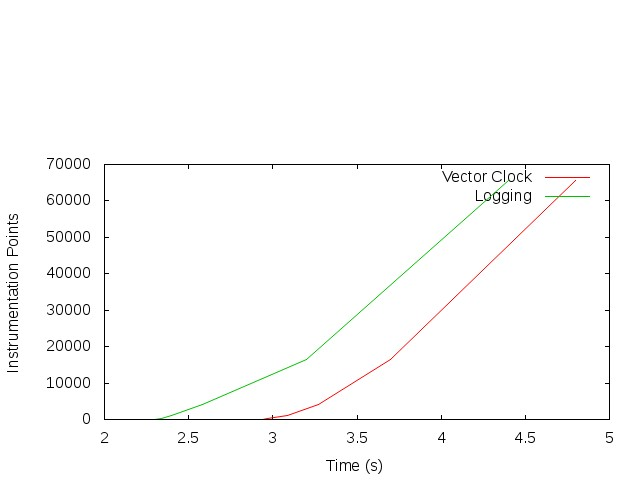
\includegraphics[width=0.50\textwidth]{fig/instrumentationTime}
%%     \caption{Instrumentation time vs \# of instrumentation points. In etcd raft}
%%     \label{fig:inst-perf}
%% \end{figure}
%%%%%%%%%%%%%%%%%%%%%%%%%%%%%%%%%%%%%%%%%%%%%%%%%%%%%%

\begin{figure}[h]
    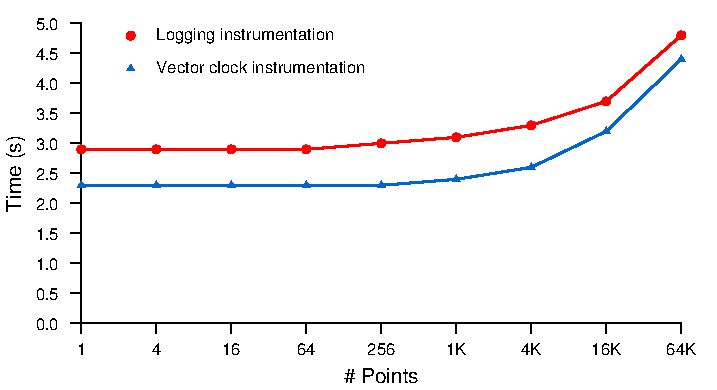
\includegraphics[width=\linewidth]{fig/raft-performance-plot}
  \caption{Time required to instrument Etcd Raft, for logging state
    and vector clocks.}
    \label{fig:inst-perf}
\end{figure}


%%%%%%%%%%%%%%%%%%%%%%%%%%%%%%%%%%%%%%%%%%%%%%%%%%%%%%
%% \begin{table}[t]
%%   \centering
%%   \small
%%   \begin{tabular}{| r | r | r |}
%%     \hline
%%     \textbf{\# Points} & \textbf{Logging (s)} & \textbf{Vector clock (s)} \\ \hline
%%     1     & 2.9 &  2.3 \\ \hline
%%     4     & 2.9 &  2.3 \\ \hline
%%     16    & 2.9 &  2.3 \\ \hline
%%     64    & 2.9 &  2.3 \\ \hline
%%     256   & 3.0 &  2.3 \\ \hline
%%     1,024  & 3.1 &  2.4 \\ \hline
%%     4,096  & 3.3 &  2.6 \\ \hline
%%     16,384 & 3.7 &  3.2 \\ \hline
%%     65,536 & 4.8 &  4.4 \\ \hline
%%   \end{tabular}
  
%%   \caption{Etcd Raft instrumentation performance table: Column 1 lists
%%     the number of instrumentation points introduced to etcd's source code. Column 2 logging
%%     code instrumentation time. Column 3 is the vector clock
%%     instrumentation time. }
%%   \label{table:inst-perf}
%% \end{table}
%%%%%%%%%%%%%%%%%%%%%%%%%%%%%%%%%%%%%%%%%%%%%%%%%%%%%%

%%%%%%%%%%%%%%%%%%%%%%%%%%%%%%%%%%
%\subsection{Logging overhead}
%\label{sec:log-overhead}
%%%%%%%%%%%%%%%%%%%%%%%%%%%%%%%%%%

\textbf{Logging overhead.} Logging state at runtime slows down the
system, possibly perturbing its execution. We instrumented etcd Raft
with increasing counts of logging statements each one logging 7
variables. We benchmarked a cluster with 3 nodes, and invoked 64
\emph{get} and 64 \emph{put} requests. Each cluster was run 3 times
and the total running time was averaged. Table~\ref{table:run-perf}
shows a linear correlation between additional logging statemens and
runtime.  The average execution time of a
single logging statement is 20 microseconds. In our local area network
with a round trip time of 0.05ms while running etcd with 1 second
timeouts we can execute approximately 50k logging statements per node
before perturbing the system.

%%%%%%%%%%%%%%%%%%%%%%%%%%%%%%%%%%%%%%%%%%%%%%%%%%%%%%
\begin{table}[t]
  \centering
  \small
  \begin{tabular}{| r | r | r | r | r|}
    \hline
    \pbox{1cm}{\textbf{Logging annotations}} & \textbf{\pbox{1.5cm}{Annotations  \\ executed}} & \pbox{1.1cm}{\textbf{Log size (MB)}} & \pbox{1cm}{\textbf{Runtime (s)}} & \textbf{\pbox{1cm}{Runtime\\overhead \%}} \\ \hline
    0 & 0 & 0  & 2.66 & 0 \\ \hline
    1 & 2.8K & 3.2 & 2.70 & 1.5 \\ \hline
    2 & 5.6K & 4.3 & 2.77 & 4.0 \\ \hline
    5 & 14K & 9.7 & 3.01 & 12.9 \\ \hline
    10 & 28K & 18.0 & 3.31 & 24.3\\ \hline
    30 & 85K & 51.7 & 4.48 & 68.0 \\ \hline
    100 & 261K & 167.9 & 7.66 & 187.5\\ \hline
  \end{tabular}
  
  \caption{Runtime performance of logging code.}
  \label{table:run-perf}
\end{table}
%%%%%%%%%%%%%%%%%%%%%%%%%%%%%%%%%%%%%%%%%%%%%%%%%%%%%%

%\begin{figure}[h]
%    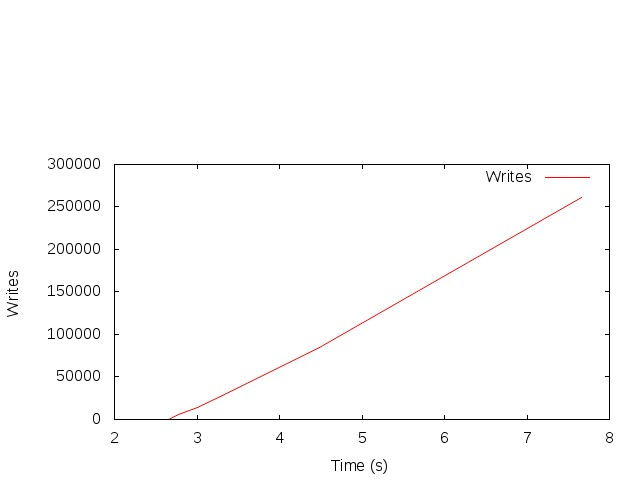
\includegraphics[width=0.50\textwidth]{fig/logsVsWrites}
%    \caption{Runtime vs logging statements executed. 
%      \iv{Is this figure graphing what is in table 4? Which column.. I can't figure this out, which is bad}
%      \iv{Time should be on the Y axis, not X axis.}
%      \iv{What is 'writes'? Rename.}
%      \iv{Drop legend}
%}
%    \label{fig:run-perf}
%\end{figure}

%%%%%%%%%%%%%%%%%%%%%%%%%%%%%%%%%%
%\subsection{Bandwidth Overhead}
%%%%%%%%%%%%%%%%%%%%%%%%%%%%%%%%%%

\textbf{Bandwidth overhead.} Vector clocks introduce bandwidth
overhead. Each entry in \dinv's vector clocks timestamp has two 32 bit
integers: one to identify the node, and the other is the node's
logical clock timestamp. The overhead of vector clocks is a product of
the number of nodes interacting during execution and the number of
messages: $64bits * nodes * messages$. In practice adding vector
clocks to messages slows down each message, which can impact the
behaviour of the system. To measure bandwidth overhead in a real
system we executed etcd Raft using the setup described above. In the
experiment we incremented the number of nodes. The bandwidths of all
nodes was aggregated together for these measurements. Adding vector
clocks to Raft slowed down the broadcast of heartbeat messages and
actually caused a \emph{reduction} in bandwidth of 10KB for all nodes
in a 4 node cluster.  As the number of nodes in the system grew, the
size of the vector clocks overcame the bandwidth saving.
Figure~\ref{fig:bandwidth-overhead} depicts the difference in
bandwidth overhead between instrumented and un-instrumented Raft
averaged over 3 runs.

%    \begin{table}[t]
%        \begin{tabular}{| p{1.5cm} | p{1.5cm} | l | l |}
%            \hline
%            Hosts & No Clocks & Clocks & Difference \\ \hline
%            3 & 335.343 & 331.337 & -4.006 \\ \hline
%            4 & 449.083 & 438.370 & -10.713 \\ \hline
%            5 & 554.671 & 555.838 & 1.166 \\ \hline
%            6 & 657.762 & 671.001 & 13.230 \\ \hline
%            7 & 765.809 & 771.160 & 5.350 \\ \hline
%        \end{tabular}
%
 %       \caption{Bandwidth Overhead in KB}
%        \label{table:bandwidth-overhead}
%    \end{table}



\begin{figure}[h]
    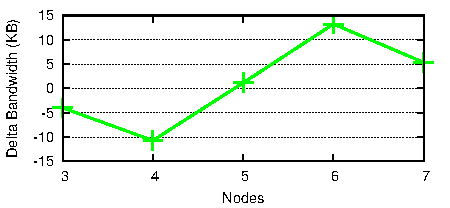
\includegraphics[width=0.50\textwidth]{fig/bandwidth-overhead}
    \caption{Difference in bandwidths between instrumented and un-instrumented etcd Raft.}
    \label{fig:bandwidth-overhead}
\end{figure}

\textbf{Dynamic analysis.} The runtime of \dinv's dynamic analysis is
affected by the size of the logs being analyzed and the number of
nodes in the execution. To measure how our performance was affected
by the length of execution we analyzed etcd Raft, and Groupcache. We
exercise both systems by issuing 10 requests per second to each system.
To demonstrate how \dinv's analysis performs with regard to
the length of execution, we analyzed the logs of 3 node clusters,
which were run for incremental intervals of 30s. Results in
Table~\ref{table:execution-vs-mergetime} show that our analysis
techniques scale linearly with the runtime of a system.  To measure
how analysis time is affected by the number of nodes in an execution
we ran etcd for 30s, exercising it with 10 client requests per second
and running clusters with incremental node counts.
Figure~\ref{fig:nodes-vs-mergetime} shows an exponential relationship
between the number of nodes and \dinv's analysis runtime.
\dinv's runtime is exponential in the number of nodes due to the
exponential growth of partial orderings our analysis techniques
compute.

\begin{table}[t]
  \centering
  \small
  \begin{tabular}{| r || r | r || r | r |}
    \hline
    \pbox{1.0cm}{\textbf{System runtime (s)}} & \textbf{\pbox{1.3cm}{Log size Raft (MB)}} & \pbox{1.1cm}{\textbf{Analysis time Raft (s)}} & \textbf{\pbox{1.3cm}{Log size GCache (MB)}} & \pbox{1.1cm}{\textbf{Analysis time GCache (s)}} \\ \hline
    30 & 5.1 & 12.7 & 0.3 & 2.8 \\ \hline
    60   & 10.5 & 28.1 & 0.3 & 3.0 \\ \hline
    90   & 13.7 & 35.9 & 1.7 & 19.6 \\ \hline
    120   & 17.4 & 48.7 & 1.4 & 21.2 \\ \hline
    150   & 22.5 & 68.8 & 1.8 & 11.3 \\ \hline
    180   & 27.7 & 99.1 & 2.1 & 18.6 \\ \hline
  \end{tabular}
  
    \caption{\dinv's dynamic analysis runtime vs the runtime of etcd
      Raft and GroupCache (GCache).}
    \label{table:execution-vs-mergetime}
\end{table}


%\begin{figure}[h]
%    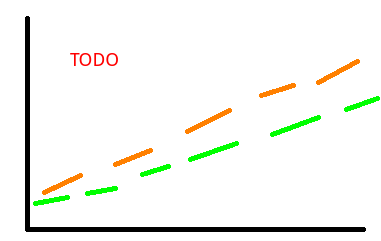
\includegraphics[width=0.50\textwidth]{fig/execution-vs-mergetime}
%    \caption{\dinv's dynamic analysis runtime vs the runtime of etcd Raft and Groupcache}
 %   \label{fig:execution-vs-mergetime}
%\end{figure}

\begin{figure}[h]
    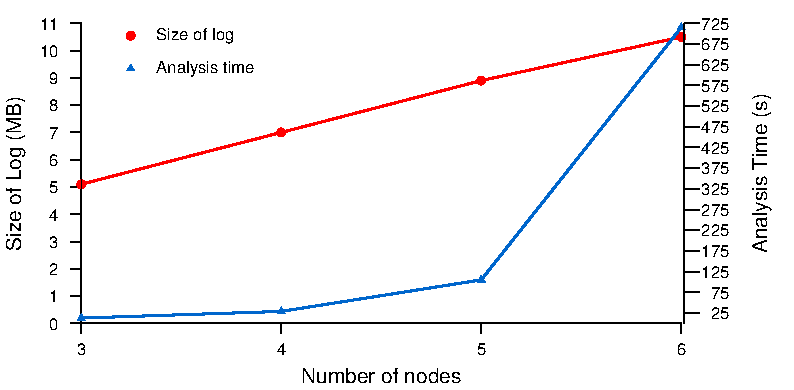
\includegraphics[width=0.50\textwidth]{fig/dynamic-analysis-runtime}
    \caption{\dinv's dynamic analysis runtime vs the number of nodes in etcd Raft}
    \label{fig:nodes-vs-mergetime}
\end{figure}

%TODO overhead benchmarks, taipei, etcd ( dump statement
%overhead, instrumentation time, log merging time, log length, dump
%statement numbers TODO TODO TODO TODO TODO



